\subsection{Атомарное key value хранилище (алгоритм ABD)}

Теперь рассмотрим применение model checker-а к нетривиальному примеру – атомарному (линеаризуемому) key-value хранилищу, использующему для репликации алгоритм ABD \cite{abd}.

Алгоритм ABD – решает задачу репликации атомарного регистра с операциями Set и Get, где Set – запись значения по ключу, Get – чтение значения по ключу. Key-value хранилище использует этот алгоритм независимо для каждого ключа.

В данном алгоритме каждая операция отправляет свои запросы на все реплики, но дожидается подтверждения лишь от большинства. Чтения и записи на большинство серверов называются кворумными.

Операция Set – двухфазная: на первой фазе выполняется чтение с кворума реплик и получение максимальной логической временной метки, на второй фазе – кворумная запись значения с выбранной на первой фазе временной меткой.

Операция Get также двухфазная: на первой фазе выполняется кворумное чтение для получения актуального значения, на второй – запись прочитанного значения с максимальной временной меткой. Вторая синхронная фаза не влияет на результат чтения, но необходима для линеаризуемости.

Чтобы model checker был полезным, он должен с одной стороны, находить ошибки в некорректных алгоритмах, а с другой – за разумное время завершать перебор всех состояний в случае корректного алгоритма.

В данном примере model checker должен найти нарушение линеаризуемости в однофазном алгоритме и подтвердить корректность двухфазного.

Клиенты будут делать одинаковые запросы для обоих видов алгоритмов. Один Getter, другой Setter. Работать оба клиента будут с одним ключем “a”. 

Изначально значение по ключу “а” пустое. Setter выполняет операцию Set(“a”, “1”). Getter выполняет последовательно две операции Get(“а”). Исполнение, которое нарушает  свойство линеаризуемости в однофазном алгоритме, устроено так, что операция Set конкурирует с обеими операциями Get.

Для данного примера применимы все эвристики. Отключение хэширования кучи, так как основное состояние – это локальное персистентное хранилище на диске. Моментальная доставка RPC ответов, потому что после отправки запроса реализация алгоритма выполняет блокирующее ожидание ответов.

Минимальный пример строится на трех репликах.

\subsubsection{Однофазный алгоритм}

Рассмотрим нарушение линеаризуемости, которое обнаруживает инструмент. Как обсуждалось выше, нам потребуется два клиента.

На рис.~\ref{fig:one_phase} изображена история доставки сообщений. Операции клиентов изображены сверху и снизу. Три прямые линии посередине – это история (временная ось) каждой из реплик для ключа “а”. Рядом с ключем пишется значение. В случае, если значение пустое, не пишется ничего.

\begin{figure}[h]
    \centering
    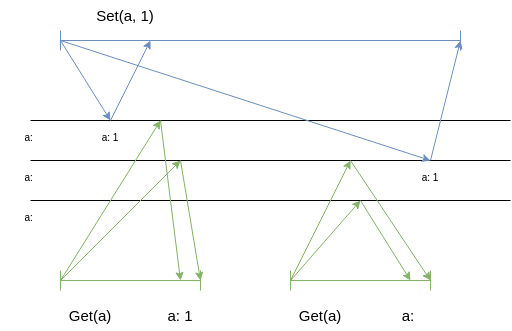
\includegraphics[width=\textwidth]{img/one_phase.png}
    \caption{История для однофазного алгоритма с нарушением линеаризуемости}
    \label{fig:one_phase}
\end{figure}

Для упрощения схемы не будем рисовать первую фазу Set с выбором временной метки, считая что клиент выполняющий Set всего один.

Клиент, дважды выполняющий Get, в результате первой операции прочитал новое значение, а в результате второй – старое. что нарушает линеаризуемость.

На поиск нарушения линеаризуемости model checker с включенными эвристиками затрачивает примерно 1 секунду и 10 MB памяти.

\subsubsection{Двухфазный алгоритм}

Также инструмент тестировался на реализации двухфазной версии алгоритма, которая не нарушает линеаризуемости.

На рис.~\ref{fig:two_phase} изображена история двухфазного алгоритма, которая нарушала свойство для однофазного алгоритма. В данном исполнении первая операция Get не будет завершена пока не произойдет запись нового значения. Это будет гарантировать, что второй Get прочтет новое значение.

\begin{figure}[h]
    \centering
    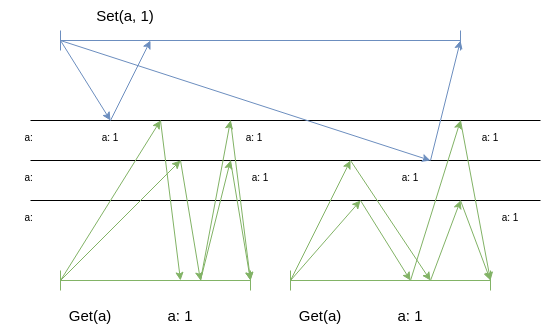
\includegraphics[width=\textwidth]{img/two_phase.png}
    \caption{История для двухфазного алгоритма}
    \label{fig:two_phase}
\end{figure}

В этой версии алгоритма через сеть будет проходить то же количество запросов, что и в однофазной версии, плюс сообщения, порожденные второй фазой операции Get. Полный перебор всех состояний с включенными эвристиками затрачивает примерно 8 минут и 20 MB памяти.
